\chapter{The birth of geometry. \cite{ueno01}}

Il capitolo ha l'obiettivo di chiarire le varie angolature da cui la geometria pu\`o essere studiata. Teniamo a mente che dal XVI secolo, le scienze, e di conseguenza la geometria e di conseguenza la matematica in generale,  vengono studiate non soltanto pi\`u dal punto di vista qualitativo ma anche quantitativo. Per quanto riguarda la geometria, questo passaggio immagino, non avendo ancora capito se vero, che si rifletta con il passaggio dalla geometria euclidea a quella cartesiana per finire a quella affine ovvero allo studio della geometria dal punto di vista della teoria degli inseiemi. Per tutti i tipi di geometria che qui imprudentemente chiamo euclidea, cartesiana e affine vi \`e alla base un sistema di assiomi che sono il punto di partenza di ogni ragionamento ed il riferimento per il modello che andremo a costruire a partire da essi.
Sarebbe bello poi concludere che della geometria cartesiana possiamo disinteressarcene ossia considerla subordinata alle altre due nel senso che essa viene utilizzata come una libreria grafica ossia per rappresentare graficamente/visivamente/senza parole le altre due geometrie. Ovvero un sistema configurabile in grado di disegnare punti, linee e curve. Forzando l'immaginazione la geometria cartesiana pu\`e essere considerato un device \cite{vonNeumann1944}. Qui non interessa solo ...

L'unica geometria che a noi dovrebbe interessare \`e quella affine (o anche geometria combinatoria. \cite{magliveras01}).

\section{Euclidean geometry}
Geometry was developed in various ancient civilizations. It was in ancient Greece that geometry apeeared in a complete form that can be regarded as the starting point of today's mathematics. Acually, geometry was developed as a practical science useful for surveying in other old civilizations, but in Greece it was also developed as an object of purely intellectual pursuit. Such developments by the school of Pythagoras had interactions with geometric views on numbers that were related to religious and philosophicals indeas. By around 300 B.C. the geometry of Euclid was presented in its complete form in the book \emph{The Elements}. It is not know whether Euclid, supposed to be author of the treatise, actually lived or not. It is certain that many mathematicians participated in its development. \textbf{The treatise includes the theory of \underline{ratios} and a geometric treatment of numbers, with geometry itself as the main theme}. \textcolor{red}{In geometry, it started from a small number of postulates and logically deduced the properties of lines, triangles, circles, etc., and was regarded as the standard model for a systematic treatise in scholarly writing for a long time to come.}

\noindent
{\color{red} \rule{\linewidth}{0.5mm} }

Although the axiomatic system for Euclidean geometry was reorganized by Hilbert and others around the turn of the 20th century, it is amazing that as early as the third and fourth centuries B.C. the method was established to deduce underlying properties of geometric objects. We could say that mathematics itself became an independent science with \emph{The Elements}.

\subsection{The Theory of Conics of Apollonius}
The so-called Euclidean geometry treated in \emph{The Elements} was concerned with lines and circles, in other words, it was the geometry of figures that can be drawn with ruler and compass. Although these objects led to interesting geometry, they were not sufficient, as was recognized in ancient Greece. 

\begin{verbatim}
http://mathworld.wolfram.com/GeometricCongruence.html
http://mathworld.wolfram.com/Isometry.html
http://planetmath.org/euclideantransformation

cite{coxeter01} Geometry revisited 1967

\end{verbatim}
TODO: FARE ESERCIZI A MANINA

% TODO - SISTEMARE DIMENSIONE IMMAGINE
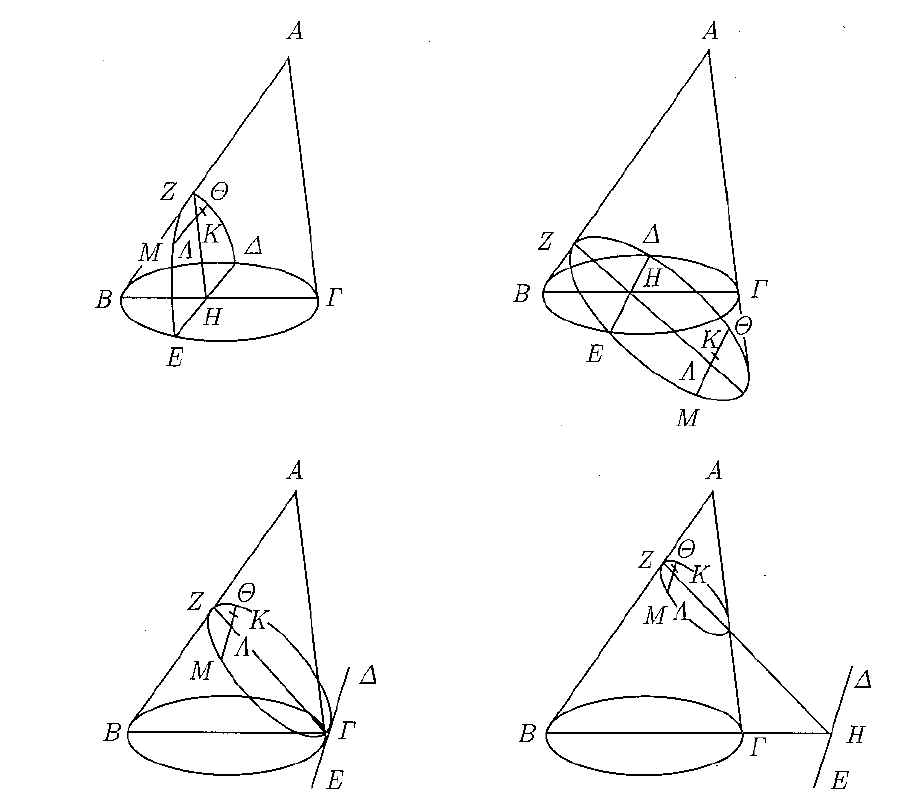
\includegraphics[width=\textwidth]{ConicsOfApollonius.png}